% Propósito: mostrar que una gráfica temporal y una fotografía espacial de la
% misma onda tienen ejes horizontales y periodicidades diferentes.
% Origen: xi(x,t)=xi_hat cos(omega t-kx+phi_0), con phi_0=0,
% f=1000 Hz, c=340 m/s, T=1.0 ms y lambda=0.340 m, como en el ejemplo
% de la sección \ref{sec:u3-ejemplo-onda}.
% Curvas teóricas normalizadas; no representan datos medidos.
% Descripción accesible: dos paneles sinusoidales. El superior muestra
% desplazamiento normalizado frente al tiempo y marca un período de 1,0 ms.
% El inferior muestra el mismo desplazamiento frente a la posición y marca una
% longitud de onda de 0,340 m. En ambos, la fase inicial es cero.
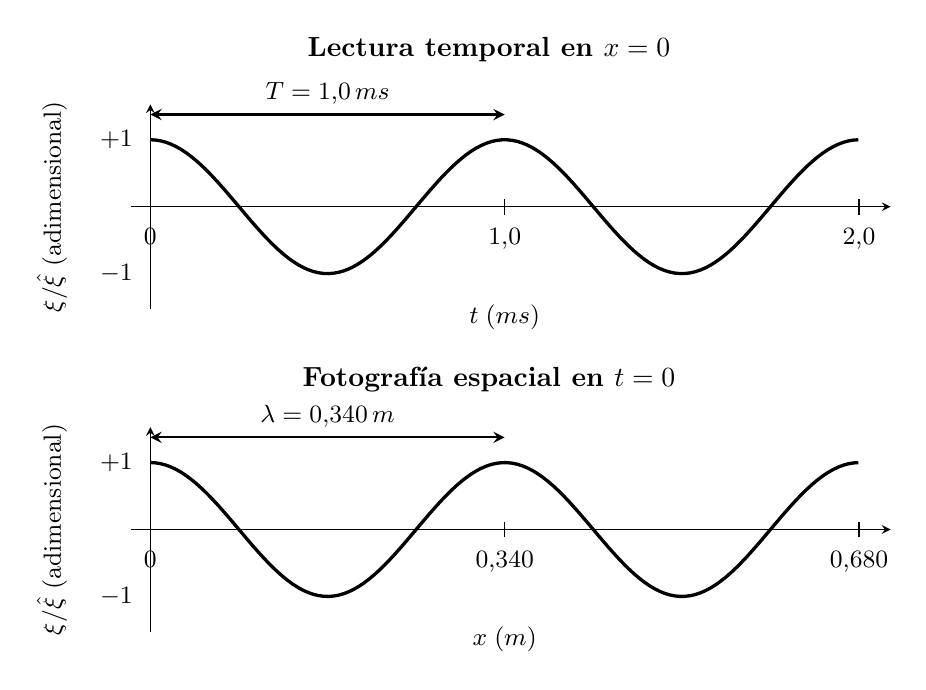
\begin{tikzpicture}[font=\small,>=stealth,x=1cm,y=1cm]
    % Panel temporal.
    \node[font=\bfseries] at (6.20,3.65)
        {Lectura temporal en \(x=0\)};
    \draw[->] (1.65,1.65) -- (11.30,1.65);
    \draw[->] (1.90,0.35) -- (1.90,2.95);
    \draw[very thick,samples=140,domain=0:2]
        plot ({1.90+4.50*\x},{1.65+0.85*cos(360*\x)});
    \node[rotate=90] at (0.65,1.65)
        {\(\xi/\hat{\xi}\) (adimensional)};
    \node at (6.40,0.25) {\(t\;(\text{ms})\)};
    \foreach \x/\lab in {0/{0},1/{1{,}0},2/{2{,}0}}{
        \pgfmathsetmacro{\xx}{1.90+4.50*\x}
        \draw (\xx,1.55) -- (\xx,1.75);
        \node[below] at (\xx,1.50) {\(\lab\)};
    }
    \node[anchor=east] at (1.80,2.50) {\(+1\)};
    \node[anchor=east] at (1.80,0.80) {\(-1\)};
    \draw[<->,thick] (1.90,2.82) -- (6.40,2.82)
        node[midway,above] {\(T=1{,}0\,\text{ms}\)};

    % Panel espacial.
    \node[font=\bfseries] at (6.20,-0.55)
        {Fotografía espacial en \(t=0\)};
    \draw[->] (1.65,-2.45) -- (11.30,-2.45);
    \draw[->] (1.90,-3.75) -- (1.90,-1.15);
    \draw[very thick,samples=140,domain=0:2]
        plot ({1.90+4.50*\x},{-2.45+0.85*cos(360*\x)});
    \node[rotate=90] at (0.65,-2.45)
        {\(\xi/\hat{\xi}\) (adimensional)};
    \node at (6.40,-3.85) {\(x\;(\text{m})\)};
    \foreach \q/\lab in {0/{0},1/{0{,}340},2/{0{,}680}}{
        \pgfmathsetmacro{\xx}{1.90+4.50*\q}
        \draw (\xx,-2.55) -- (\xx,-2.35);
        \node[below] at (\xx,-2.60) {\(\lab\)};
    }
    \node[anchor=east] at (1.80,-1.60) {\(+1\)};
    \node[anchor=east] at (1.80,-3.30) {\(-1\)};
    \draw[<->,thick] (1.90,-1.28) -- (6.40,-1.28)
        node[midway,above] {\(\lambda=0{,}340\,\text{m}\)};
\end{tikzpicture}
